% 模板文件
\documentclass[12pt,a4paper]{article}
\usepackage{ctex}
\usepackage{amsmath,amssymb,amsthm}
\usepackage{geometry}
\geometry{margin=2.4cm}
\usepackage{tikz}
\usetikzlibrary{angles,quotes}
% 定义定理环境
\newtheorem*{model}{模型}
\newtheorem*{proofdemo}{证明}
\begin{document}
	\title{初二上几何模型：三垂直家族 \& 半角模型}
	\author{}
	\date{}
	\maketitle


\section{一、一线三直角（三垂直 / K 型全等）}
\begin{model}
条件：点 $B,A,C$ 在同一直线上，$\angle B=\angle EAC=\angle C=90^\circ$，$AE=AC$。
\begin{center}
\begin{tikzpicture}[scale=0.9]
\coordinate (B) at (0,0);
\coordinate (A) at (2,0);
\coordinate (C) at (5,0);
\coordinate (E) at (2,3);
\draw (B)--(A)--(C);
\draw (B)--(E)--(C);
% 直角标记
\draw[thin] (2,0.2)--(2.2,0.2)--(2.2,0);
\draw[thin] (0,0.2)--(0.2,0.2)--(0.2,0);
\draw[thin] (5,0.2)--(4.8,0.2)--(4.8,0);
\node[below] at (B) {$B$};
\node[below] at (A) {$A$};
\node[below] at (C) {$C$};
\node[above] at (E) {$E$};
\end{tikzpicture}
\end{center}
结论：$\triangle ABE \cong \triangle ECA\ (\text{AAS})$，$AB=EC,\ BE=AC$。
\end{model}

\begin{proofdemo}
$\because \angle B=90^\circ$，$\therefore \angle B+\angle BEA=90^\circ$。
又 $\because \angle EAC=90^\circ$，$\therefore \angle BEA+\angle CAE=90^\circ$，
$\therefore \boldsymbol{\angle BEA=\angle CAE}$。
\[
\begin{cases}
\angle B=\angle C\\
\angle BEA=\angle CAE\\
AE=AC
\end{cases}
\]
$\therefore \triangle ABE \cong \triangle ECA\ (\text{AAS})$。
$\therefore AB=EC,\ BE=AC$。
\end{proofdemo}


\section{二、正方形半角模型（$90^\circ$ 含 $45^\circ$）}
\begin{model}
条件：正方形 $ABCD$，点 $E$ 在 $BC$ 上，点 $F$ 在 $CD$ 上，$\angle EAF=45^\circ$。
\begin{center}
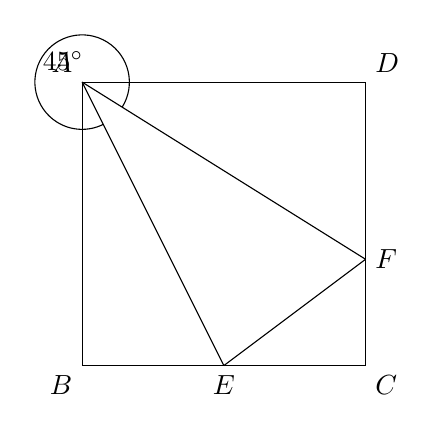
\begin{tikzpicture}[scale=0.9]
\coordinate (A) at (0,4);
\coordinate (B) at (0,0);
\coordinate (C) at (4,0);
\coordinate (D) at (4,4);
\coordinate (E) at (2,0);
\coordinate (F) at (4,1.5);
\draw (A)--(B)--(C)--(D)--cycle;
\draw (A)--(E);
\draw (A)--(F);
\draw (E)--(F);
\pic [draw, "$45^\circ$", angle radius=0.6cm] {angle = F--A--E};
\node[above left] at (A) {$A$};
\node[below left] at (B) {$B$};
\node[below right] at (C) {$C$};
\node[above right] at (D) {$D$};
\node[below] at (E) {$E$};
\node[right] at (F) {$F$};
\end{tikzpicture}
\end{center}
主结论：$\boldsymbol{EF=BE+DF}$。

推论：
\begin{enumerate}
\item $\triangle CEF$ 的周长：$C_{\triangle CEF}=2AB$；
\item $AE$ 平分 $\angle BEF$，$AF$ 平分 $\angle DFE$；
\item $S_{\triangle ABE}+S_{\triangle ADF}=S_{\triangle AEF}$；
\item 延长线版本（$E,F$ 在边延长线上）：$EF=|BE-DF|$。
\end{enumerate}
\end{model}

\begin{proofdemo}
延长 $CB$ 到 $G$，使 $BG=DF$，连接 $AG$。
\begin{center}
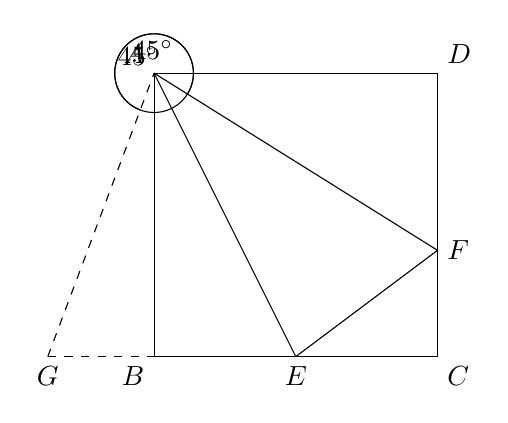
\begin{tikzpicture}[scale=0.9]
\coordinate (A) at (0,4);
\coordinate (B) at (0,0);
\coordinate (C) at (4,0);
\coordinate (D) at (4,4);
\coordinate (E) at (2,0);
\coordinate (F) at (4,1.5);
\coordinate (G) at (-1.5,0);
\draw (A)--(B)--(C)--(D)--cycle;
\draw (A)--(E);
\draw (A)--(F);
\draw (E)--(F);
\draw[dashed] (G)--(A);
\draw[dashed] (G)--(E);
\pic [draw, "$45^\circ$", angle radius=0.5cm] {angle = F--A--E};
\pic [draw, "$45^\circ$", angle radius=0.5cm] {angle = E--A--G};
\node[above left] at (A) {$A$};
\node[below left] at (B) {$B$};
\node[below right] at (C) {$C$};
\node[above right] at (D) {$D$};
\node[below] at (E) {$E$};
\node[right] at (F) {$F$};
\node[below] at (G) {$G$};
\end{tikzpicture}
\end{center}
$\because$ 四边形 $ABCD$ 是正方形，
$\therefore AB=AD,\angle ABC=\angle D=\angle BAD=90^\circ$，
$\therefore \angle ABG=\angle D=90^\circ$。
\[
\begin{cases}
AB=AD\\
\angle ABG=\angle D\\
BG=DF
\end{cases}
\]
$\therefore \triangle ABG \cong \triangle ADF\ (\text{SAS})$。
$\therefore AG=AF,\angle BAG=\angle DAF$。

$\because \angle EAF=45^\circ,\angle BAD=90^\circ$，
$\therefore \angle BAE+\angle DAF=45^\circ$，
$\therefore \angle BAE+\angle BAG=\angle GAE=45^\circ$，
即 $\boldsymbol{\angle GAE=\angle EAF=45^\circ}$。
\[
\begin{cases}
AG=AF\\
\angle GAE=\angle FAE\\
AE=AE
\end{cases}
\]
$\therefore \triangle AGE \cong \triangle AFE\ (\text{SAS})$。
$\therefore EF=GE=BG+BE=DF+BE$，即 $EF=BE+DF$。
\end{proofdemo}


\section{三、等腰直角三角形半角模型（拓展）}
\begin{model}
条件：$\triangle ABC$ 为等腰直角三角形，$AB=AC,\angle BAC=90^\circ$，$D,E$ 在 $BC$ 上，$\angle DAE=45^\circ$。
\begin{center}
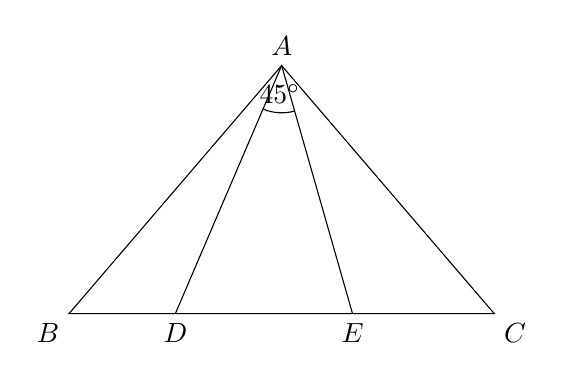
\begin{tikzpicture}[scale=0.9]
\coordinate (A) at (0,3.5);
\coordinate (B) at (-3,0);
\coordinate (C) at (3,0);
\coordinate (D) at (-1.5,0);
\coordinate (E) at (1,0);
\draw (A)--(B)--(C)--cycle;
\draw (A)--(D);
\draw (A)--(E);
\pic [draw, "$45^\circ$", angle radius=0.6cm] {angle = D--A--E};
\node[above] at (A) {$A$};
\node[below left] at (B) {$B$};
\node[below right] at (C) {$C$};
\node[below] at (D) {$D$};
\node[below] at (E) {$E$};
\end{tikzpicture}
\end{center}
结论：$\boldsymbol{DE^2=BD^2+EC^2}$。
\end{model}

\begin{proofdemo}
将 $\triangle ABD$ 绕点 $A$ 逆时针旋转 $90^\circ$ 得到 $\triangle ACG$，连接 $EG$。
\begin{center}
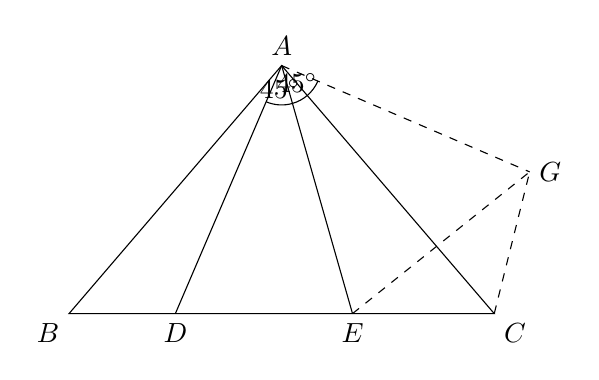
\begin{tikzpicture}[scale=0.9]
\coordinate (A) at (0,3.5);
\coordinate (B) at (-3,0);
\coordinate (C) at (3,0);
\coordinate (D) at (-1.5,0);
\coordinate (E) at (1,0);
\coordinate (G) at (3.5,2);
\draw (A)--(B)--(C)--cycle;
\draw (A)--(D);
\draw (A)--(E);
\draw[dashed] (A)--(G);
\draw[dashed] (C)--(G);
\draw[dashed] (E)--(G);
\pic [draw, "$45^\circ$", angle radius=0.5cm] {angle = D--A--E};
\pic [draw, "$45^\circ$", angle radius=0.5cm] {angle = E--A--G};
\node[above] at (A) {$A$};
\node[below left] at (B) {$B$};
\node[below right] at (C) {$C$};
\node[below] at (D) {$D$};
\node[below] at (E) {$E$};
\node[right] at (G) {$G$};
\end{tikzpicture}
\end{center}
易证 $\triangle ABD\cong\triangle ACG$，$BD=CG,\angle B=\angle ACG=45^\circ$，
$\therefore \angle ECG=\angle ACB+\angle ACG=90^\circ$，$\triangle ECG$ 是直角三角形，
$\therefore EG^2=CG^2+EC^2=BD^2+EC^2$。
再证 $\triangle ADE\cong\triangle AGE(\text{SAS})$，得 $DE=EG$，
$\therefore DE^2=BD^2+EC^2$。
\end{proofdemo}

\end{document}
